\documentclass[11pt,a4paper]{article}

\usepackage[utf8]{inputenc}
\usepackage[T1]{fontenc}
\usepackage[slovak,english]{babel}
\usepackage[a4paper,margin=2.3cm]{geometry}
\usepackage{lmodern}
\usepackage{amsmath}
\usepackage{booktabs}
\usepackage{array}
\usepackage{tabularx}
\usepackage{graphicx}
\usepackage{float}
\usepackage{xcolor}
\usepackage{hyperref}
\usepackage{enumitem}
\usepackage{microtype}

\definecolor{darkblue}{RGB}{25,55,95}
\hypersetup{colorlinks=true,linkcolor=darkblue,urlcolor=darkblue}
\setlength{\parindent}{0pt}
\setlength{\parskip}{0.55em}
\renewcommand{\arraystretch}{1.2}
\newcolumntype{Y}{>{\raggedright\arraybackslash}X}

\title{Parametrizácia genetického algoritmu\\\large Umelá inteligencia 2 -- Zadanie č. 1}
\author{}
\date{24. september 2026}

\begin{document}
\selectlanguage{slovak}
\maketitle

\section{Nastavenie experimentu}

Experimenty boli vykonané pomocou genetického algoritmu nad knižnicou
\texttt{genetic\_all}. Každá konfigurácia bola spustená šesťkrát s rôznymi
random seedmi (42 až 47). Pri minimalizačnej úlohe platí, že menšia
fitness je lepšia.

\begin{table}[H]
\centering
\caption{Spoločné nastavenie experimentov}
\begin{tabular}{ll}
\toprule
Populácia & 50 jedincov \\
Počet premenných & 10 \\
Počet generácií & 250 (bonus Eggholder: 2000) \\
Počet behov konfigurácie & 6 \\
Výber & turnajový \texttt{seltourn} alebo náhodný \texttt{selrand} \\
Kríženie & \texttt{crossov}, jednobodové \\
Elitizmus & \texttt{selsort}, najlepší jedinci prenesení bez zmeny \\
\bottomrule
\end{tabular}
\end{table}

Hlavnou testovanou funkciou bola 10-rozmerná Schwefelova funkcia s doménou
$[-500,500]$. Jej globálne optimum je približne $f^*=-4189.83$. Jedna generácia
prebieha v poradí: elitizmus, výber rodičov, kríženie, globálna mutácia
(\texttt{mutx}) a lokálna mutácia (\texttt{muta}).

\section{Selektívny tlak a diverzita}

Selektívny tlak určuje, ako silno sú zvýhodnené kvalitné jedince. Nastavoval som
ho typom výberu a počtom elitných jedincov. Pri turnajovom výbere z dvoch náhodných
jedincov vždy postúpi lepší, pri náhodnom výbere fitness vôbec nerozhoduje.

Diverzita určuje, ako intenzívne algoritmus skúša nové oblasti priestoru riešení.
Nastavoval som ju intenzitou mutácií: \texttt{mutx\_rate} je podiel génov, ktoré
dostanú úplne novú náhodnú hodnotu z celého intervalu, \texttt{muta\_rate} je
podiel génov s malým posunom a \texttt{amp} je maximálna veľkosť tohto posunu.

\begin{table}[H]
\centering
\caption{Testované úrovne selektívneho tlaku a diverzity}
\begin{tabularx}{\textwidth}{lYY}
\toprule
 & \textbf{Selektívny tlak} & \textbf{Diverzita} \\
\midrule
Veľký & turnajový výber \texttt{seltourn} a elitizmus 3 jedincov &
$\texttt{mutx\_rate}=0.15$, $\texttt{muta\_rate}=0.25$, $\texttt{amp}=60$ \\
Malý & náhodný výber \texttt{selrand} a bez elitizmu &
$\texttt{mutx\_rate}=0.01$, $\texttt{muta\_rate}=0.02$, $\texttt{amp}=5$ \\
\bottomrule
\end{tabularx}
\end{table}

\begin{table}[H]
\centering
\caption{Parametre variantov a--e}
\begin{tabular}{clcccc}
\toprule
Variant & Výber & Elitizmus & \texttt{mutx\_rate} & \texttt{muta\_rate} & \texttt{amp} \\
\midrule
a & \texttt{seltourn} & 3 & 0.15 & 0.25 & 60 \\
b & \texttt{seltourn} & 3 & 0.01 & 0.02 & 5 \\
c & \texttt{selrand}  & 0 & 0.15 & 0.25 & 60 \\
d & \texttt{selrand}  & 0 & 0.01 & 0.02 & 5 \\
e & \texttt{seltourn} & 1 & 0.05 & 0.08 & 20 \\
\bottomrule
\end{tabular}
\end{table}

\subsection{Experimenty a--e}

\begin{figure}[H]
\centering
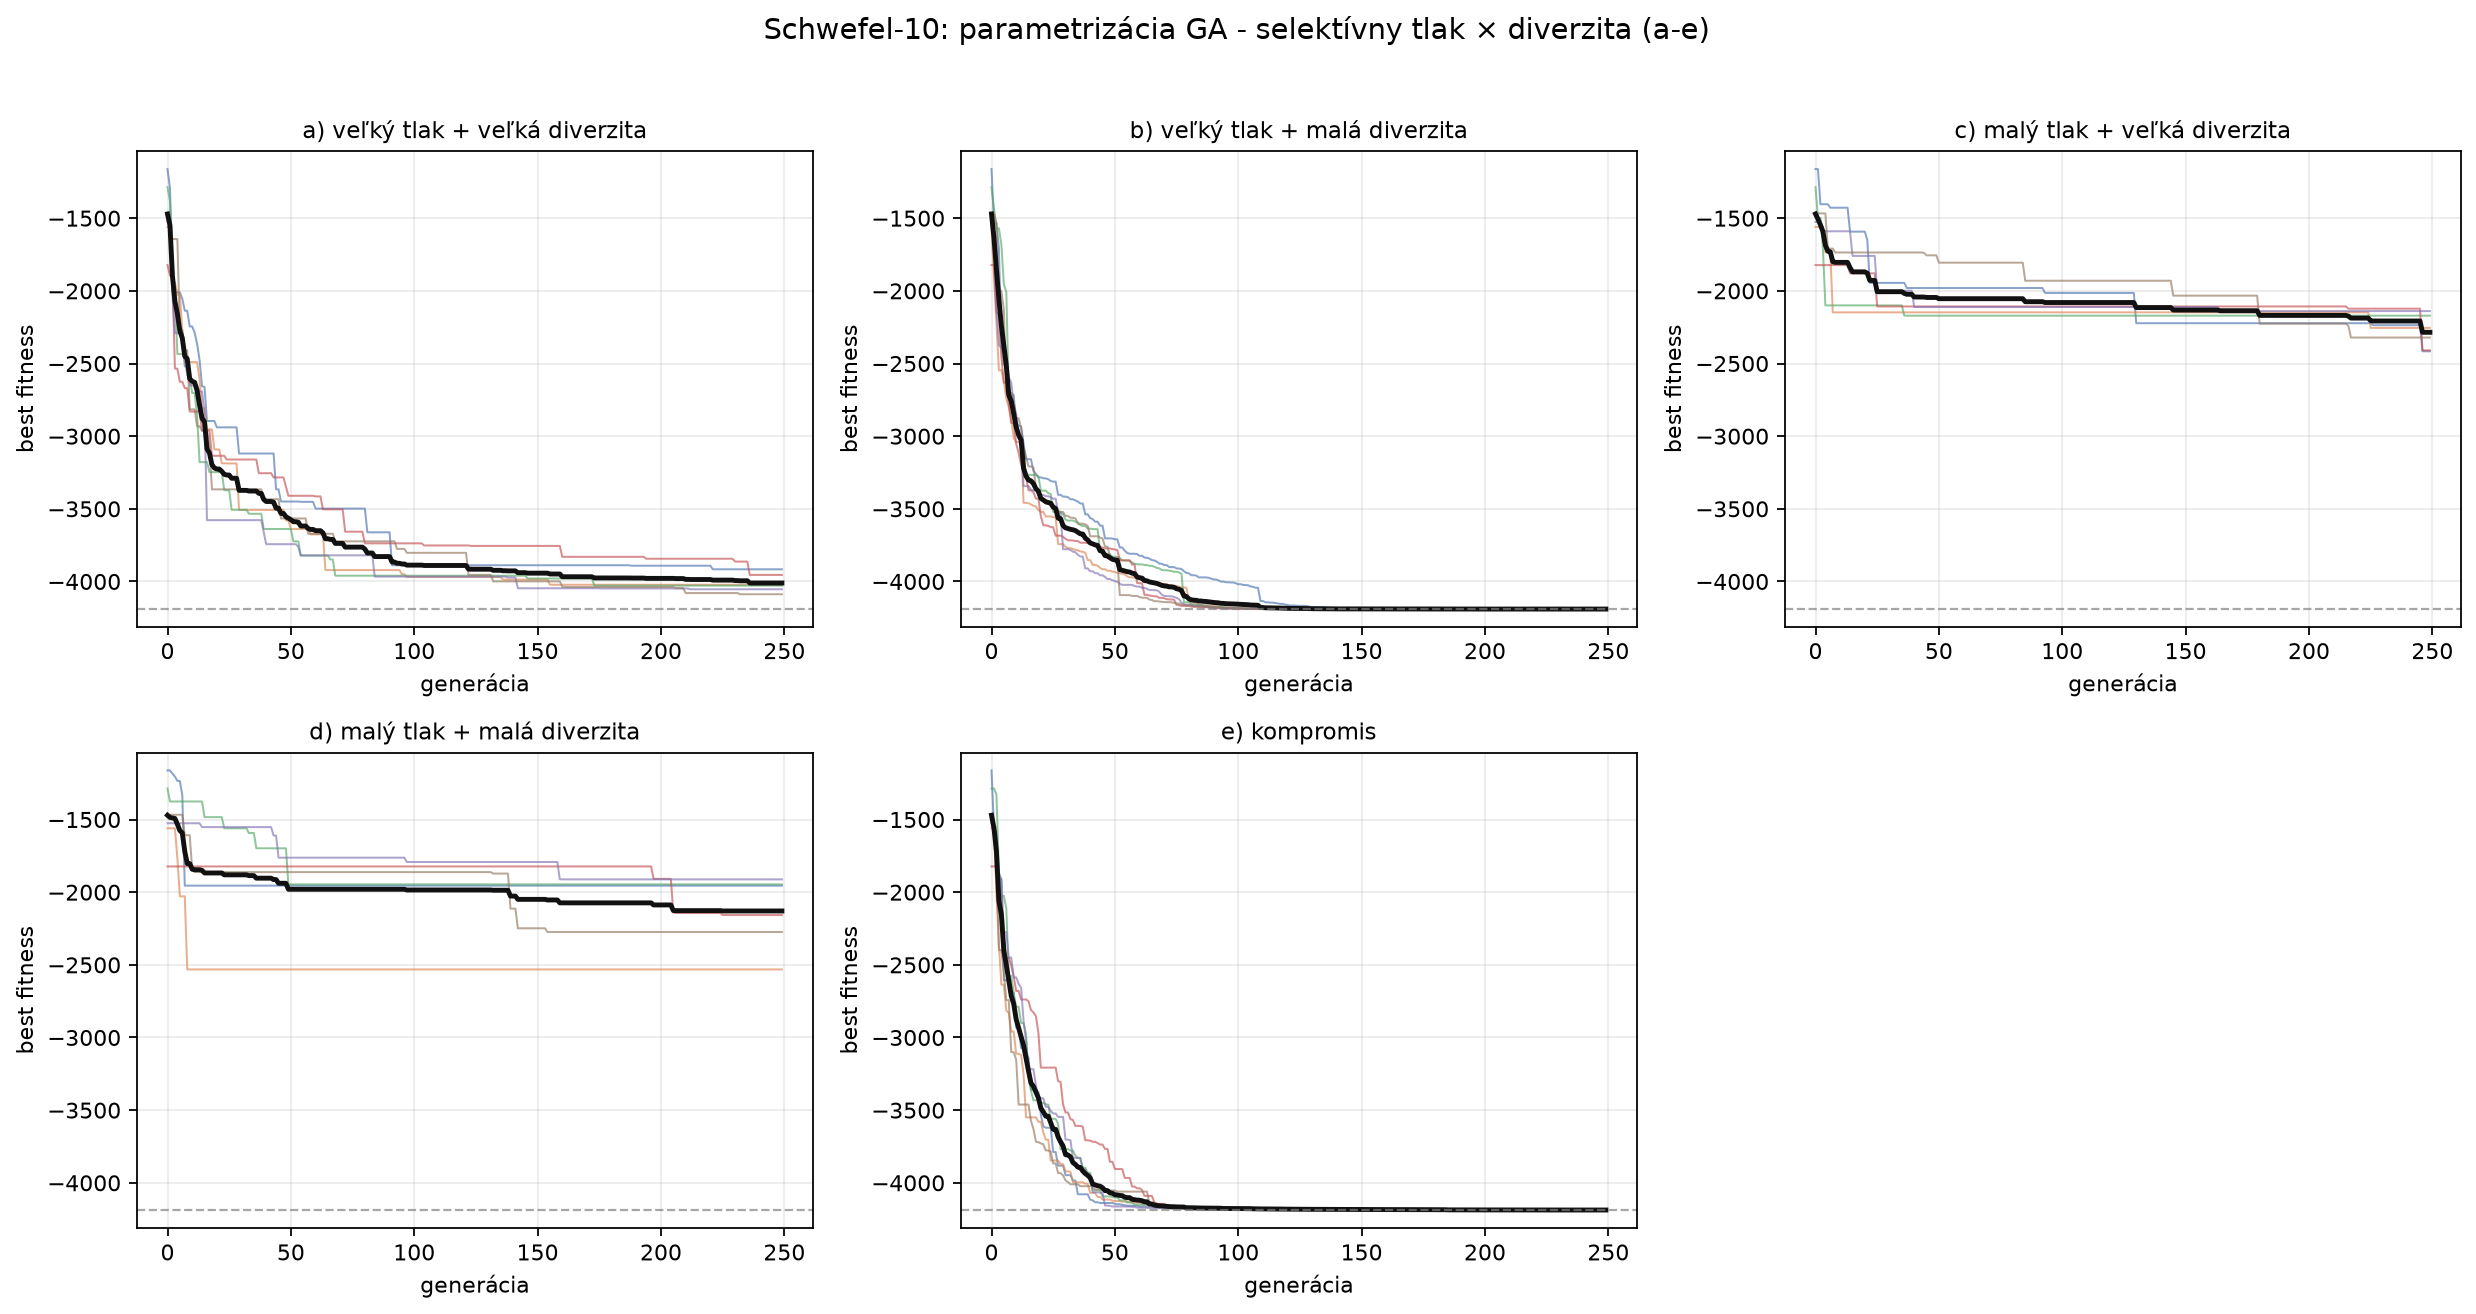
\includegraphics[width=\textwidth]{results/fig1_schwefel_a_e.png}
\caption{Schwefel-10, varianty a--e. Farebne 6 behov, čierna je ich priemer,
prerušovaná čiara je globálne minimum.}
\end{figure}

\begin{table}[H]
\centering
\small
\caption{Najlepšia fitness na konci jednotlivých behov, Schwefel-10}
\begin{tabular}{ccccccc|cc}
\toprule
Variant & beh 1 & beh 2 & beh 3 & beh 4 & beh 5 & beh 6 & najlepší & priemer \\
\midrule
a & $-3916.2$ & $-4022.4$ & $-4028.4$ & $-3954.9$ & $-4053.6$ & $-4087.7$ & $-4087.71$ & $-4010.52$ \\
b & $-4189.8$ & $-4189.8$ & $-4189.8$ & $-4189.8$ & $-4189.8$ & $-4189.8$ & $\mathbf{-4189.83}$ & $\mathbf{-4189.82}$ \\
c & $-2415.9$ & $-2255.0$ & $-2170.8$ & $-2409.3$ & $-2139.3$ & $-2321.4$ & $-2415.92$ & $-2285.28$ \\
d & $-1955.0$ & $-2531.6$ & $-1946.2$ & $-2157.5$ & $-1912.0$ & $-2274.0$ & $-2531.64$ & $-2129.38$ \\
e & $-4188.6$ & $-4188.1$ & $-4185.2$ & $-4187.4$ & $-4185.6$ & $-4188.6$ & $-4188.64$ & $-4187.26$ \\
\bottomrule
\end{tabular}
\end{table}

Hranicu $-4000$ prekonali varianty a, b aj e. Najväčší rozdiel spôsobuje
selektívny tlak, nie samotná diverzita. Varianty a a b s turnajovým výberom a
elitizmom rýchlo konvergujú a dostávajú sa blízko globálneho optima. Pri
variantoch c a d sa bez tlaku na lepších jedincov algoritmus správa podobne ako
náhodné prehľadávanie a končí okolo $-2100$ až $-2500$.

V rámci konfigurácií s veľkým tlakom bol lepší variant b s menšou diverzitou,
ktorý našiel globálne minimum vo všetkých 6 behoch. Silné mutácie vo variante a
po nájdení dobrého riešenia zbytočne narúšajú populáciu, preto sa nedostane
úplne do optima. Pri malom tlaku sa rozdiel diverzity výrazne neprejaví, pretože
kvalitné gény sa nedokážu v populácii presadiť.

Graf zobrazuje najlepšieho jedinca nájdeného od začiatku behu, preto sú krivky
monotónne. Pri variantoch c a d bez elitizmu sa môže najlepší jedinec v populácii
medzi generáciami aj zhoršiť, v grafe to však nie je vidieť.

\section{Kompromisný variant e}

Variant e používa miernejší, ale stále účinný tlak a strednú diverzitu:
turnajový výber, elitizmus jedného jedinca, $\texttt{mutx\_rate}=0.05$,
$\texttt{muta\_rate}=0.08$ a $\texttt{amp}=20$.

Priemerný výsledok bol $-4187.3$, teda prakticky rovnaký ako pri extrémnejšom
variante b. Variant e však konverguje rýchlejšie (približne do 70. generácie,
b až okolo 120. generácie) a ponecháva si viac diverzity, čo sa ukázalo
užitočné pri členitejšej Eggholderovej funkcii.

\section{Vypínanie operátorov (f--i)}

V experimentoch f--i bol z kompromisného variantu e postupne odstránený jeden
alebo oba operátory.

\begin{figure}[H]
\centering
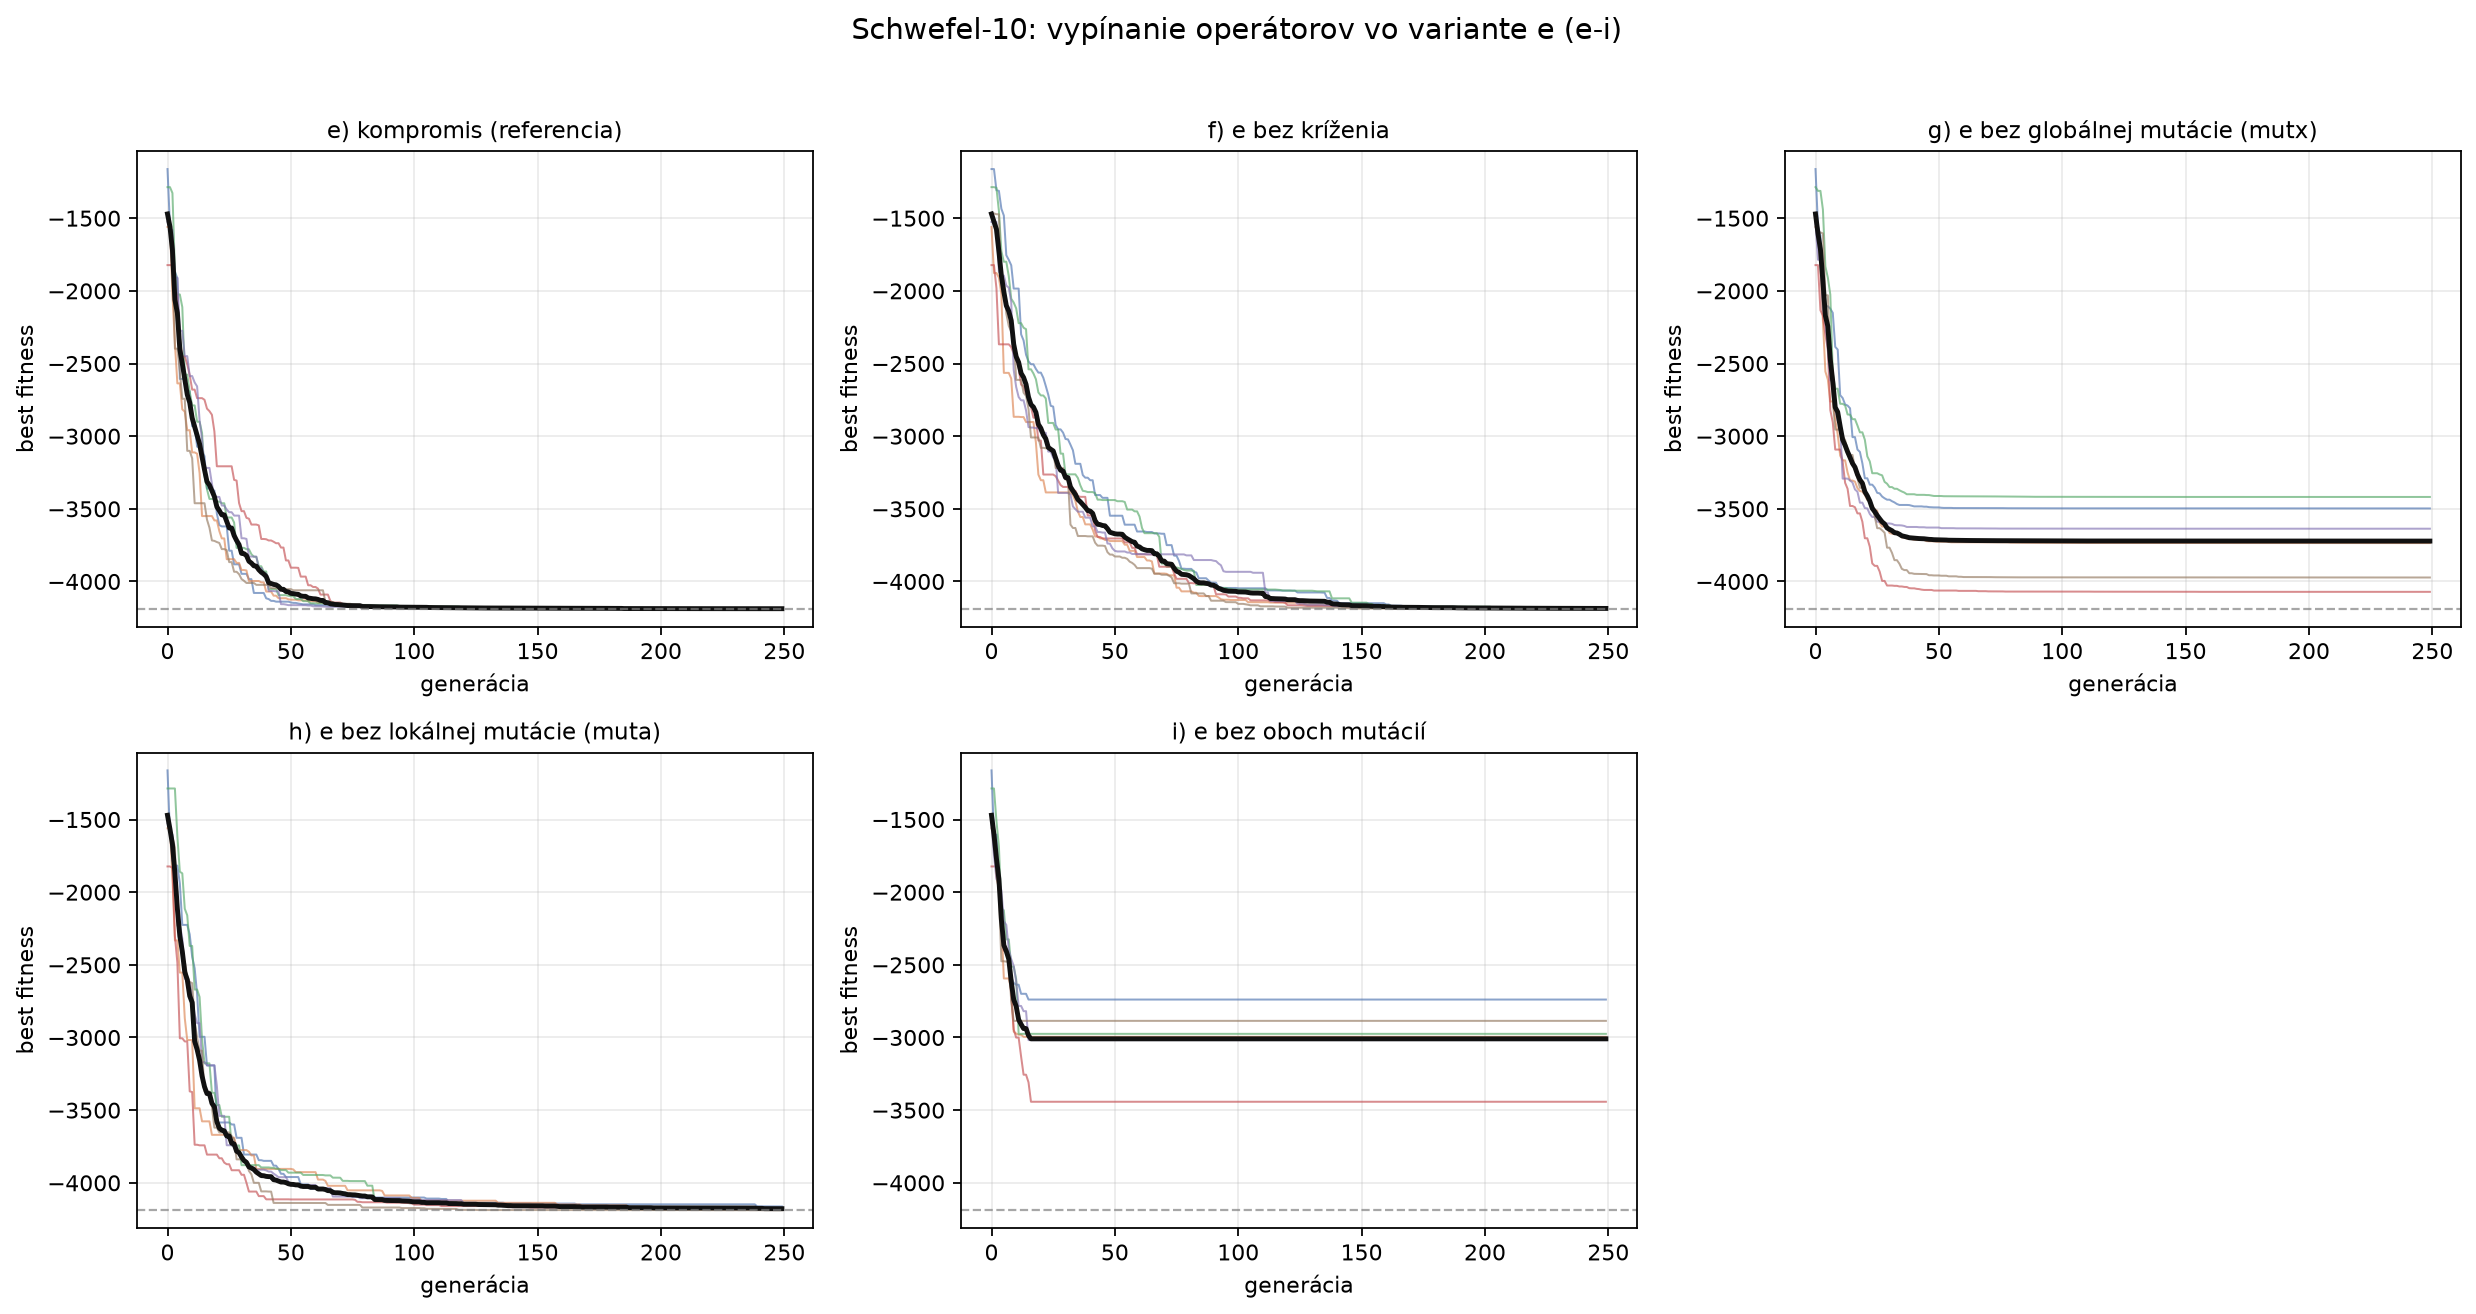
\includegraphics[width=\textwidth]{results/fig2_schwefel_e_i.png}
\caption{Schwefel-10, variant e a jeho úpravy f--i.}
\end{figure}

\begin{table}[H]
\centering
\small
\caption{Najlepšia fitness na konci jednotlivých behov, varianty e--i}
\begin{tabular}{ccccccc|cc}
\toprule
Variant & beh 1 & beh 2 & beh 3 & beh 4 & beh 5 & beh 6 & najlepší & priemer \\
\midrule
e & $-4188.6$ & $-4188.1$ & $-4185.2$ & $-4187.4$ & $-4185.6$ & $-4188.6$ & $-4188.64$ & $-4187.26$ \\
f & $-4184.1$ & $-4186.6$ & $-4178.3$ & $-4188.3$ & $-4188.1$ & $-4187.4$ & $-4188.33$ & $-4185.47$ \\
g & $-3497.4$ & $-3735.7$ & $-3418.4$ & $-4071.3$ & $-3636.9$ & $-3972.6$ & $-4071.33$ & $-3722.03$ \\
h & $-4162.8$ & $-4179.2$ & $-4180.0$ & $-4182.2$ & $-4175.1$ & $-4188.7$ & $-4188.67$ & $-4178.01$ \\
i & $-2738.9$ & $-2995.3$ & $-2974.9$ & $-3442.2$ & $-3018.0$ & $-2885.5$ & $-3442.20$ & $-3009.14$ \\
\bottomrule
\end{tabular}
\end{table}

\begin{itemize}[leftmargin=1.5em]
  \item \textbf{f -- bez kríženia:} konečný výsledok je takmer rovnaký ako pri e,
  ale konvergencia je asi dvakrát pomalšia (okolo 150. generácie namiesto 70.).
  Schwefelova funkcia je separovateľná, takže mutácie dokážu prehľadávať gény
  samostatne, kríženie hlavne urýchľuje šírenie dobrých génov.
  \item \textbf{g -- bez globálnej mutácie:} všetky behy sa zasekli v lokálnych
  minimách už okolo 50. generácie, priemer klesol z $-4187.3$ na $-3722.0$.
  \item \textbf{h -- bez lokálnej mutácie:} iba malý pokles ($-4178.0$), jemné
  doladenie je pomalšie, ale globálna mutácia a kríženie ho čiastočne nahradia.
  \item \textbf{i -- bez oboch mutácií:} najhorší výsledok ($-3009.1$). Populácia
  stratí diverzitu približne za 20 generácií a kríženie už len skladá tie isté gény.
\end{itemize}

Najdôležitejším operátorom je globálna mutácia \texttt{mutx}. Tá nahrádza gén
náhodnou hodnotou z celého povoleného intervalu, umožňuje veľké skoky, udržuje
diverzitu a pomáha opustiť lokálne minimá.

\section{Bonus: Eggholder-10}

Varianty a--e boli otestované na 10-rozmernej Eggholderovej funkcii s doménou
$[-512,512]$. Eggholder je oveľa členitejšia a susedné premenné $x_j$ a $x_{j+1}$
sú na sebe závislé. Pri 250 generáciách bol najlepší beh variantu e len
$-7595.5$, preto som počet generácií zvýšil na 2000 a variant e doladil:
3-bodové kríženie, $\texttt{muta\_rate}=0.2$ a menšia amplitúda $\texttt{amp}=5$
(častejšie, ale jemnejšie posuny). Globálna mutácia zostala $0.05$. Varianty a--d
majú rovnaké parametre ako pri Schwefelovej funkcii.

\begin{figure}[H]
\centering
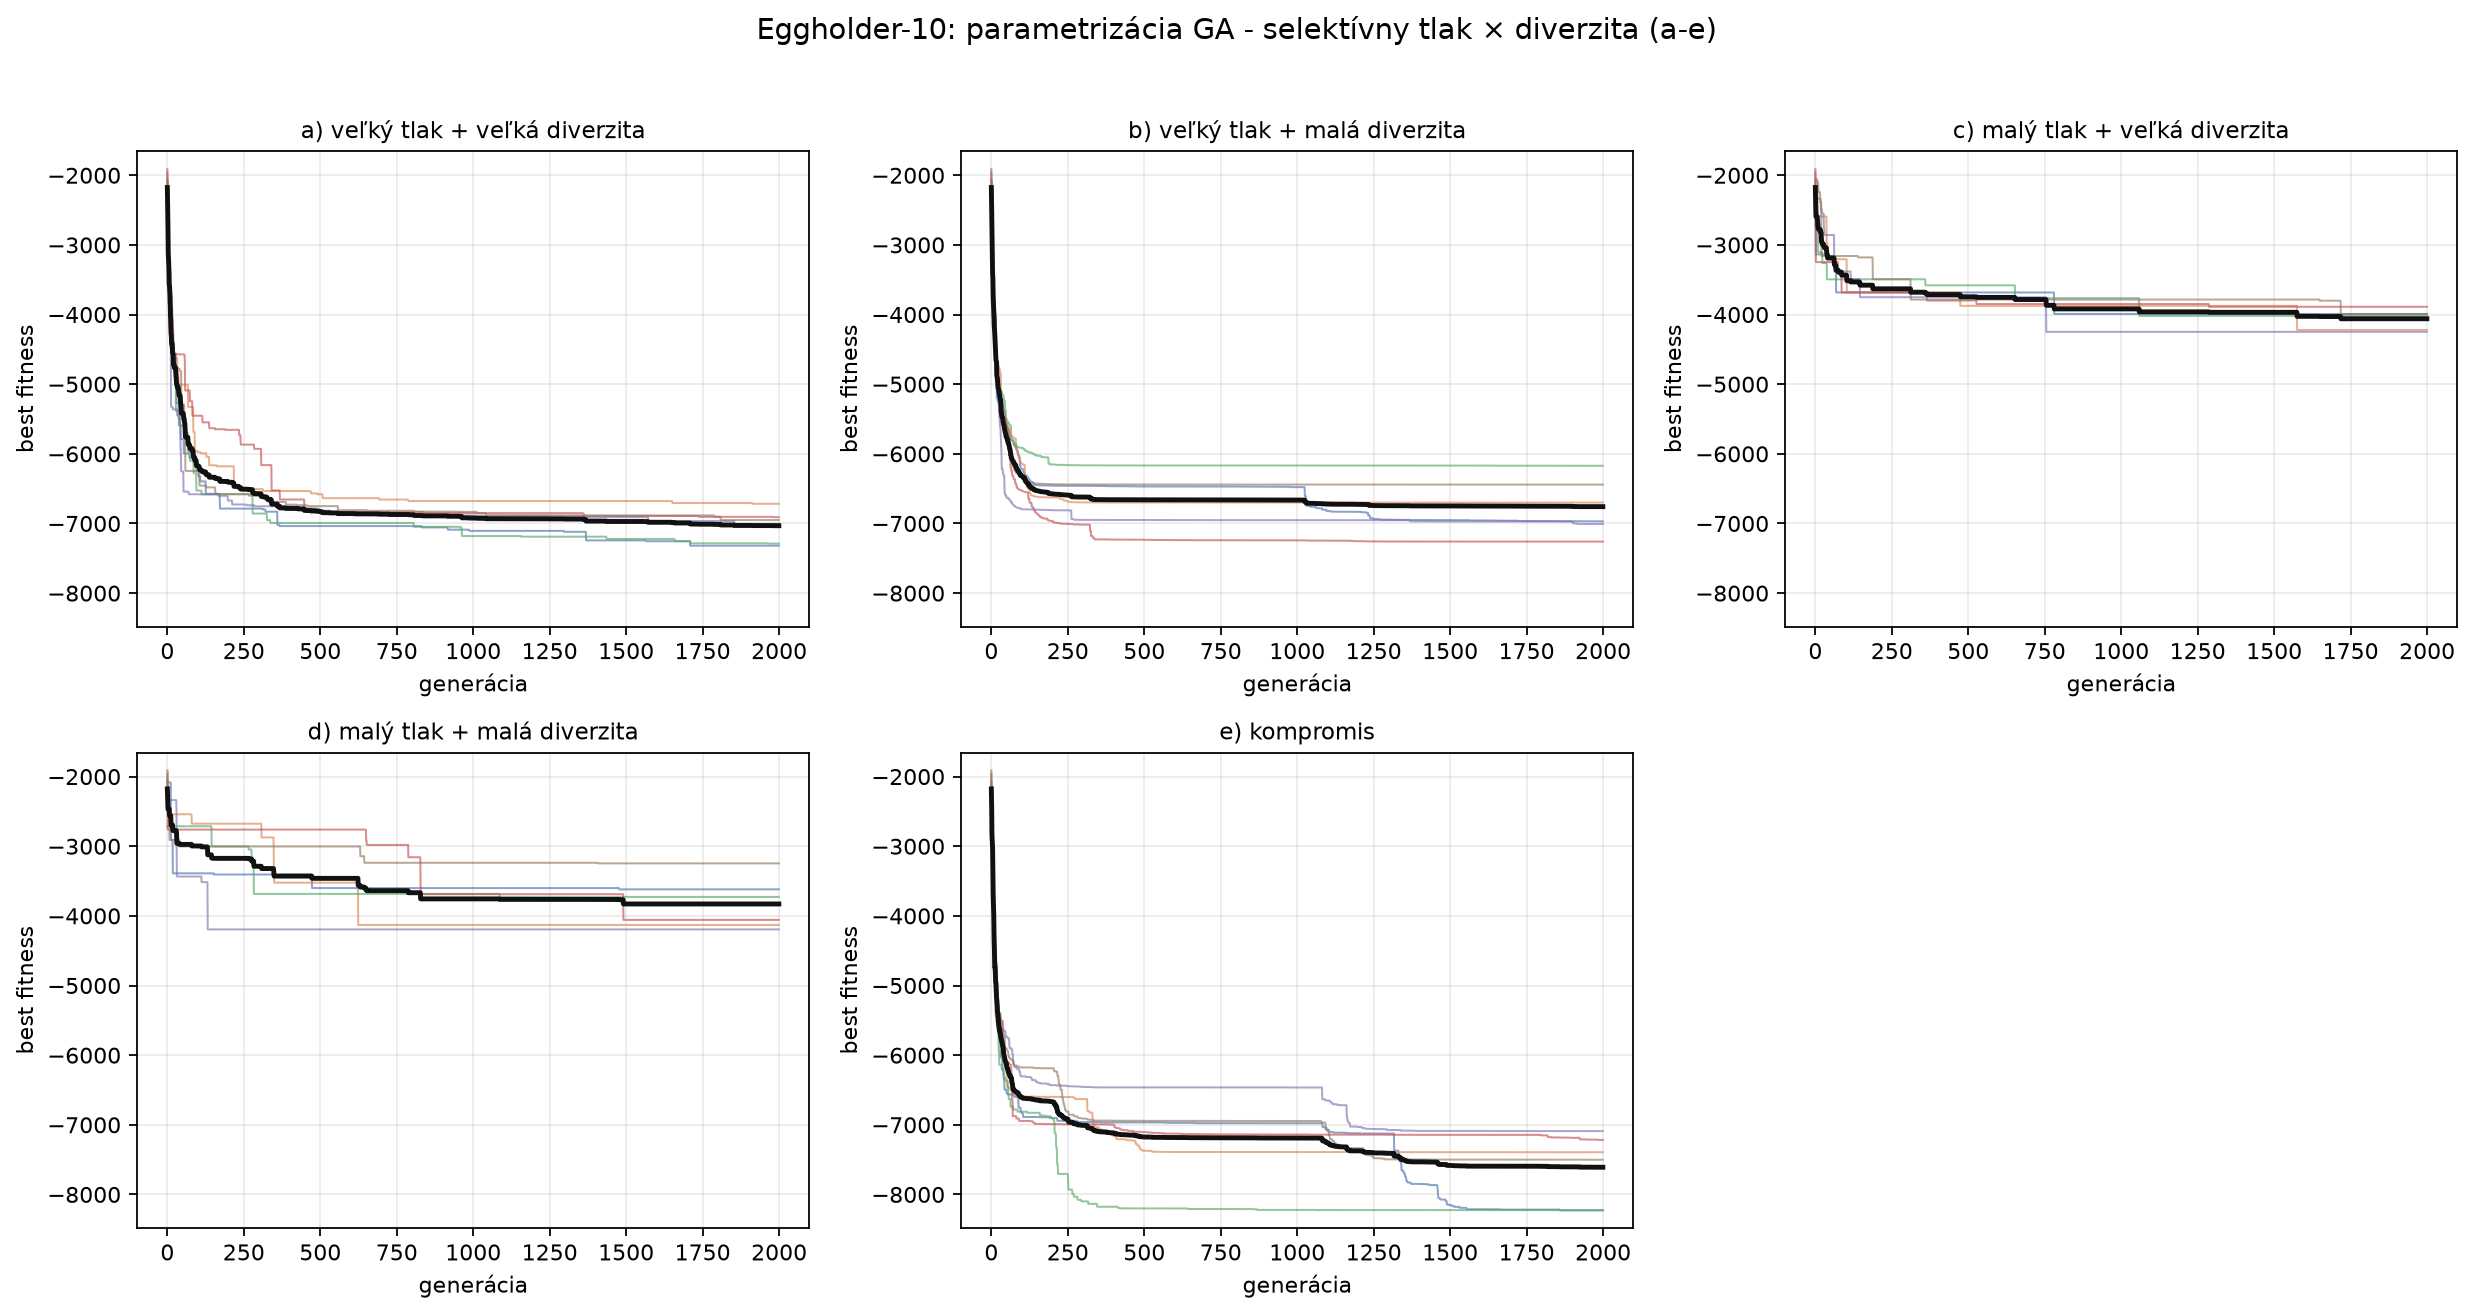
\includegraphics[width=\textwidth]{results/fig3_eggholder_a_e.png}
\caption{Eggholder-10, varianty a--e, 2000 generácií.}
\end{figure}

\begin{table}[H]
\centering
\small
\caption{Najlepšia fitness na konci jednotlivých behov, Eggholder-10}
\begin{tabular}{ccccccc|cc}
\toprule
Variant & beh 1 & beh 2 & beh 3 & beh 4 & beh 5 & beh 6 & najlepší & priemer \\
\midrule
a & $-7319.1$ & $-6716.8$ & $-7289.1$ & $-6910.7$ & $-7005.1$ & $-6950.7$ & $-7319.11$ & $-7031.91$ \\
b & $-6969.3$ & $-6699.5$ & $-6171.4$ & $-7260.6$ & $-7007.5$ & $-6442.0$ & $-7260.58$ & $-6758.37$ \\
c & $-3991.6$ & $-4221.3$ & $-4019.6$ & $-3888.6$ & $-4248.5$ & $-3993.2$ & $-4248.45$ & $-4060.48$ \\
d & $-3619.3$ & $-4130.0$ & $-3727.4$ & $-4057.6$ & $-4194.3$ & $-3246.0$ & $-4194.28$ & $-3829.12$ \\
e & $\mathbf{-8229.0}$ & $-7394.1$ & $\mathbf{-8225.1}$ & $-7216.9$ & $-7090.4$ & $-7501.6$ & $\mathbf{-8228.97}$ & $\mathbf{-7609.51}$ \\
\bottomrule
\end{tabular}
\end{table}

\begin{table}[H]
\centering
\caption{Porovnanie Schwefel-10 a Eggholder-10}
\begin{tabular}{ccccc}
\toprule
Variant & Schwefel najlepší & Schwefel priemer & Eggholder najlepší & Eggholder priemer \\
\midrule
a & $-4087.7$ & $-4010.5$ & $-7319.1$ & $-7031.9$ \\
b & $-4189.8$ & $-4189.8$ & $-7260.6$ & $-6758.4$ \\
c & $-2415.9$ & $-2285.3$ & $-4248.5$ & $-4060.5$ \\
d & $-2531.6$ & $-2129.4$ & $-4194.3$ & $-3829.1$ \\
e & $-4188.6$ & $-4187.3$ & $-8229.0$ & $-7609.5$ \\
\bottomrule
\end{tabular}
\end{table}

Najlepší beh variantu e dosiahol $-8229.0$, hranicu $-8000$ prekonali 2 zo 6
behov. Poradie variantov je podobné ako pri Schwefelovej funkcii: veľký
selektívny tlak (a, b, e) je výrazne lepší ako malý (c, d). Rozdiel je v tom, že
na Eggholderovej funkcii variant b už optimum spoľahlivo nenájde a najlepší je
doladený kompromis e. Pri separovateľnej Schwefelovej funkcii stačí silná
selekcia, pri Eggholderovej treba viac diverzity a dlhší beh. Absolútne hodnoty
fitness medzi funkciami priamo porovnávať nemožno, pretože majú odlišný tvar a mierku.

\section{Záver}

Selektívny tlak mal na rýchlosť a kvalitu konvergencie väčší vplyv než
zvolená úroveň diverzity. Najlepšie výsledky na Schwefelovej funkcii poskytli
konfigurácie s turnajovým výberom a elitizmom, variant b a kompromis e sa dostali
prakticky do globálneho minima $-4189.83$. Z jednotlivých operátorov bola
najdôležitejšia globálna mutácia \texttt{mutx}, ktorá zabezpečuje diverzitu a
umožňuje opúšťať lokálne minimá. Na Eggholderovej funkcii bol najlepší doladený
variant e s výsledkom $-8229.0$.

\end{document}
